\subsection{Сравнение особенностей конструкций с аналогами}
В данном разделе будет проведен обзор существующих аналогов систем лазерной гравировки и их конструктивных особенностей. 
Сравнение различных решений позволит выявить преимущества и недостатки каждой из них, а также обосновать 
выбор компонентов и технологий, используемых в данном курсовом проекте.

\subsubsection{WATTSAN micro 0203.}
Лазерный станок WATTSAN 0203 micro (рис. \ref{fig:wattsan}) предназначен для хобби и мелкосерийного производства.
Настольный гравер имеет рабочее поле 200×300 мм, тем самым подходит для обработки небольших изделий.
Станок достаточно компактный, поэтому может быть размещен даже при дефиците свободного пространства.
По умолчанию поставляется с лазерной трубкой мощностью 40w.

Аппарат подключается к компьютеру через USB порт и поддерживает программы CorelDraw и AutoCAD. 
Данный лазерный гравер поддерживает следующие графические форматы: BMP, PLT, CDR, DXF, AI, SVG и другие.
Станок режет фанеру до 3 мм, а акрил, оргстекло, ткань, резину, кожу и прочие материалы толщиной до 5 мм. 
Гравер не обрабатывает металл и не подходит для печатей по ГОСТУ.
\begin{figure}[ht]
    \centering
    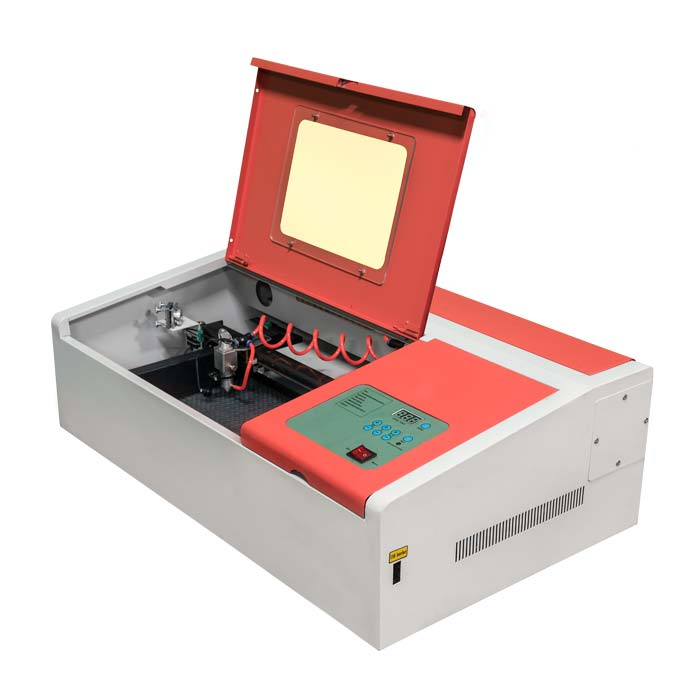
\includegraphics[width=0.6\linewidth]{\commonSecPathPrefix/sec_1/content/wattsan.jpg}
    \caption{Лазерный гравер WATTSAN micro 0203}
    \label{fig:wattsan}
\end{figure}

WATTSAN micro 0203 может использоваться для следующих целей:
\begin{itemize}
    \item Изготовление печатей;
    \item Изготовление сувениров;
    \item Гравировка на мобильных телефонах;
    \item Заготовки для творчества.
\end{itemize}

На момент написания курсовой работы, стоимость устройства в РБ составляет 3033 BYN.

\subsubsection{ORTUR Laser Master 2 S2.}
Максимальная мощность установки -- 10 Вт. Размер сжатой точки составляет 0,05 x 0,1 мм. 
Максимальная площадь гравировки -- 390*410 мм. 
Имеет пять защитных функций: обнаружение наклона, мониторинг USB-подключения, ограничение времени воздействия лазера, 
активный контроль положения лазера, система контроля напряжения и тока.
ORTUR Laser Master 2 S2 (рис. \ref{fig:ortur}) может резать акрил толщиной 30 мм и дерево толщиной 20 мм.
\begin{figure}[ht]
    \centering
    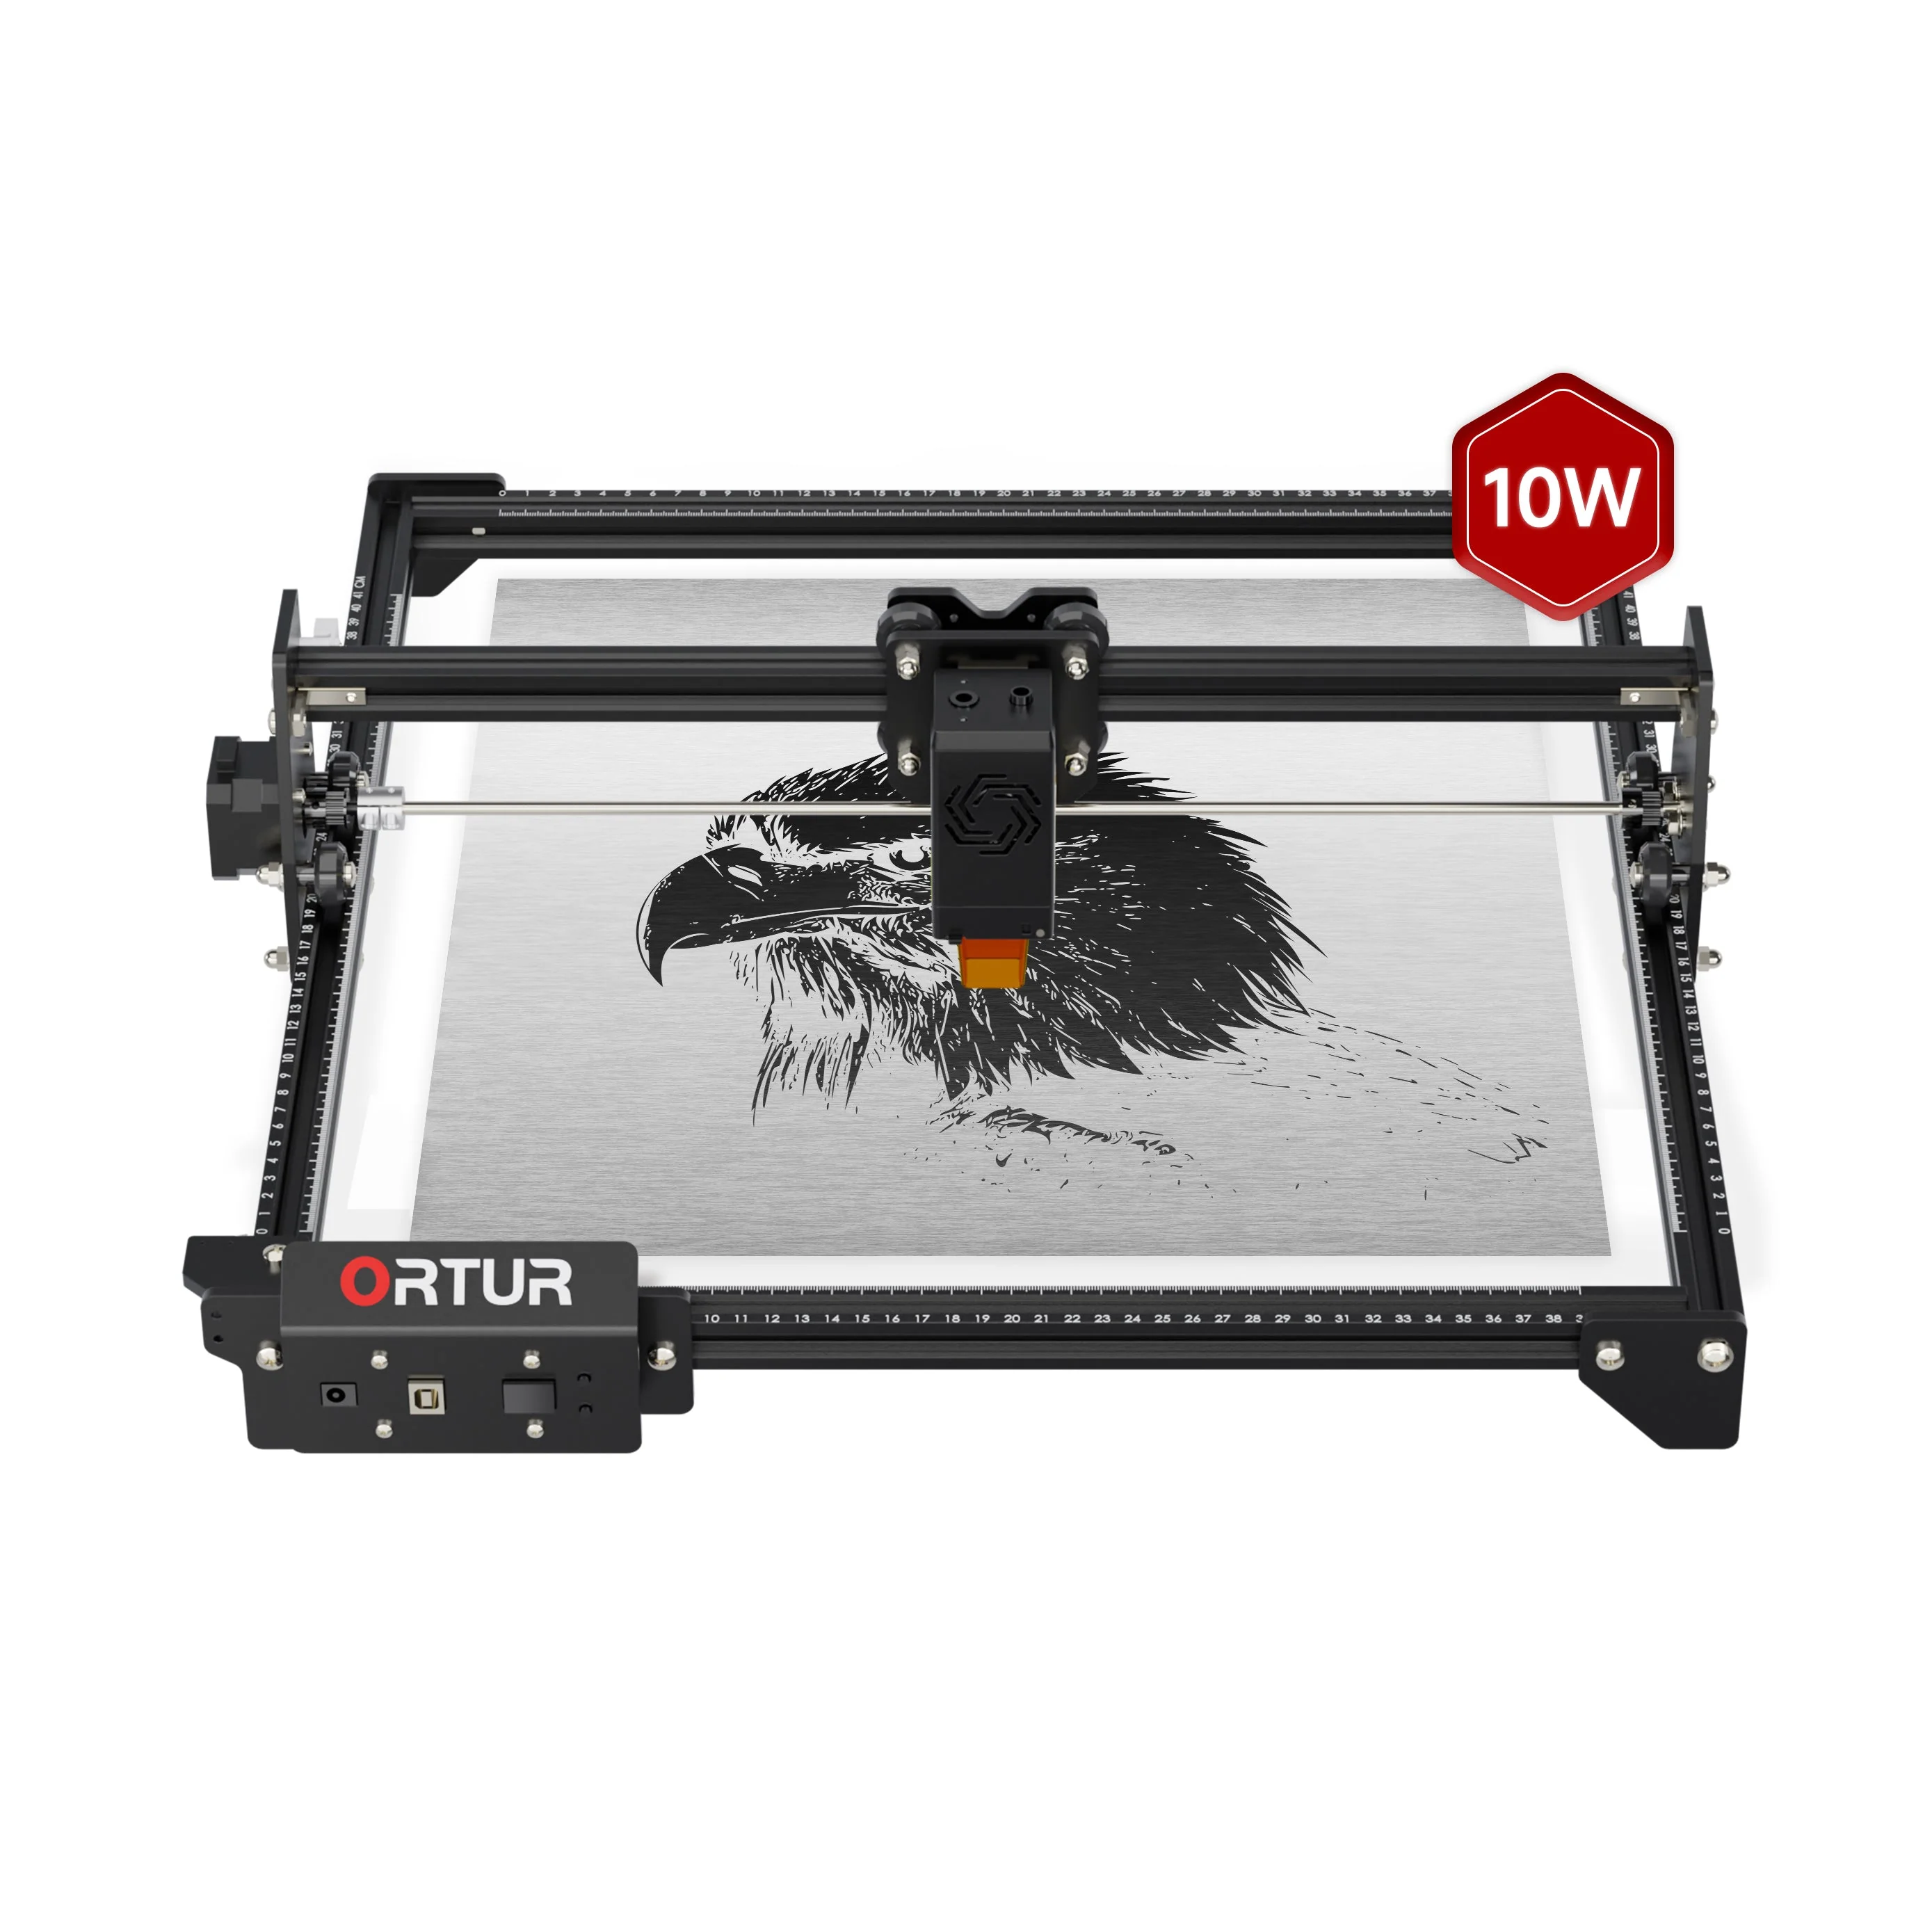
\includegraphics[width=0.6\linewidth]{\commonSecPathPrefix/sec_1/content/ortur.png}
    \caption{Гравировальный станок ORTUR Laser Master 2 S2}
    \label{fig:ortur}
\end{figure}

Лазерный гравировальный станок совместим с различными системами и программами для гравировки, такими как LaserGRBL и MAC (LightBurn). 
Программное обеспечение поддерживает следущие форматы файла гравировки: NC, DXF, BMP, JPG, JPEG, PNG, GCODE, SVG, TIF и CR2.
Данный станок имеет разнообразные области применения: возможна гравировка на бумаге, бамбуке, дереве, коже, 
оксиде алюминия, стекле и более чем 100 видах материалов.

На момент написания курсовой работы, стоимость устройства в РБ составляет 786 BYN.

\subsubsection{Two Trees TTS 55 Pro.}
Лазерный модуль обладает мощностью 5,5 Вт. Технология сжатого пятна использует линзу FAC — 
функцию коллимационного света, которая делает лазерный луч более концентрированным, 
а плотность мощности намного выше. Материнская плата устройства — 
новая 32-битная материнская плата, работающая с плавным ременным приводом, обеспечивает 
высокоскоростную гравировку до 30000 мм/мин. 
Лазерный источник гравера управляется технологией LD+FAC+C-Lens, размер пятна составляет всего 0,08 мм.
TTS 55 Pro (рис. \ref{fig:tt}) способен резать древесину толщиной 8 мм.
\begin{figure}[ht]
    \centering
    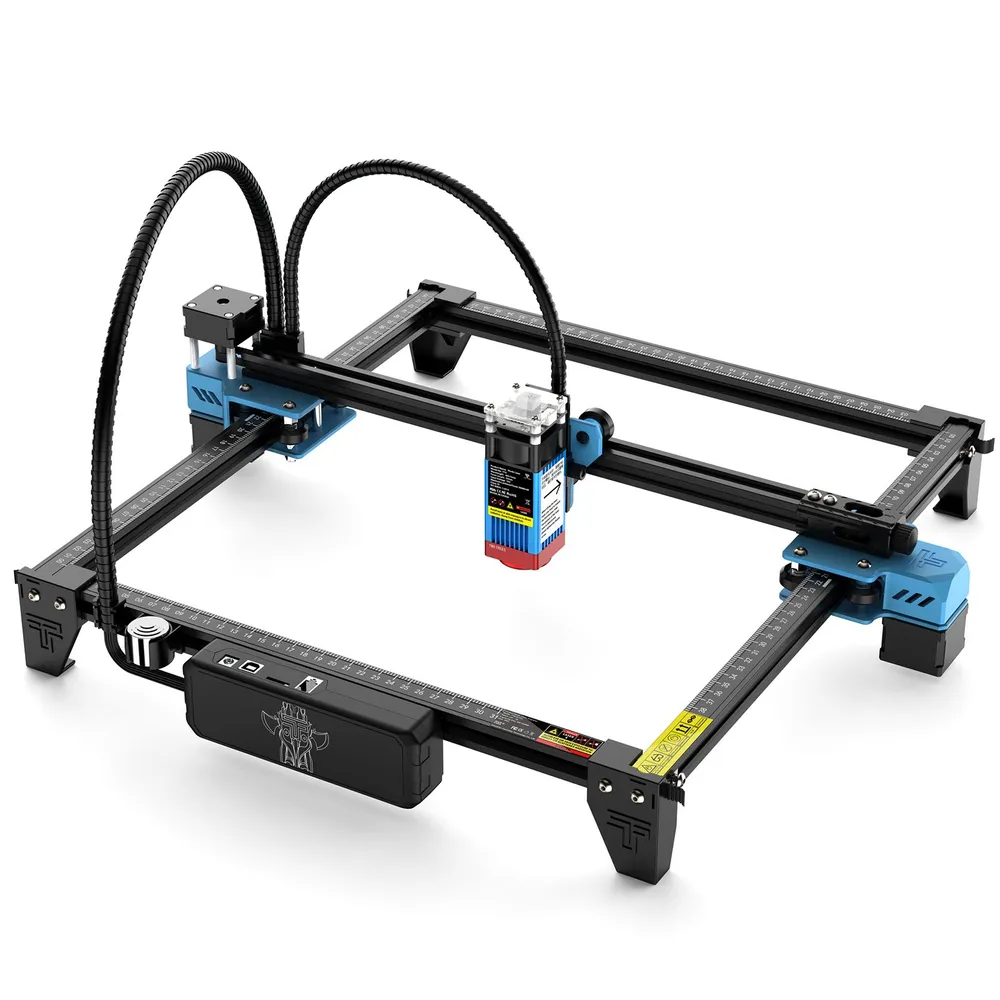
\includegraphics[width=0.6\linewidth]{\commonSecPathPrefix/sec_1/content/tt.png}
    \caption{Лазерный гравер Two Trees TTS 55 Pro}
    \label{fig:tt}
\end{figure}

Интеллектуальный модуль станка ESP32 объединяет функции Wi-Fi и BT, 
что делает его более удобным в использовании за счет поддержки подключения к приложению.
TTS-55 совместим со следующими системами и программами для гравировки: LaserGRBL и MAC (LightBurn).
Программное обеспечение поддерживает следущие форматы файла гравировки: NC, DXF, BMP, JPG, JPEG, PNG, GCODE, SVG, TIF и CR2.

TTS-55 Pro может гравировать дерево, пластик, бумагу, кожу, бамбук, оксид алюминия, нержавеющую сталь, акрил и другие. 
Лазер может разрезать фанеру толщиной до 5 мм, акриловый лист толщиной 3 мм, картон толщиной 3 мм, кожу толщиной 0,7 мм.

На момент написания курсовой работы, стоимость устройства в РБ составляет 765 BYN.